%!TEX TS-program = pdflatex
\documentclass{mycv}

\begin{document}
	\thispagestyle{plain}
	\begin{minipage}{.7\textwidth}
		\begin{flushleft}
			\name{Christos Dalamagkas}{Research Assistant}{Network Engineer}
			\contact{(+30) 698 316 0295}{cdalamagkas@gmail.com}{chris.dal}{https://christos.pw}{linkedin.com/in/cdalamagkas}{cdalamagkas}
			\birth
		\end{flushleft}
	\end{minipage}
	\begin{minipage}{.3\textwidth}
		\begin{flushright}
			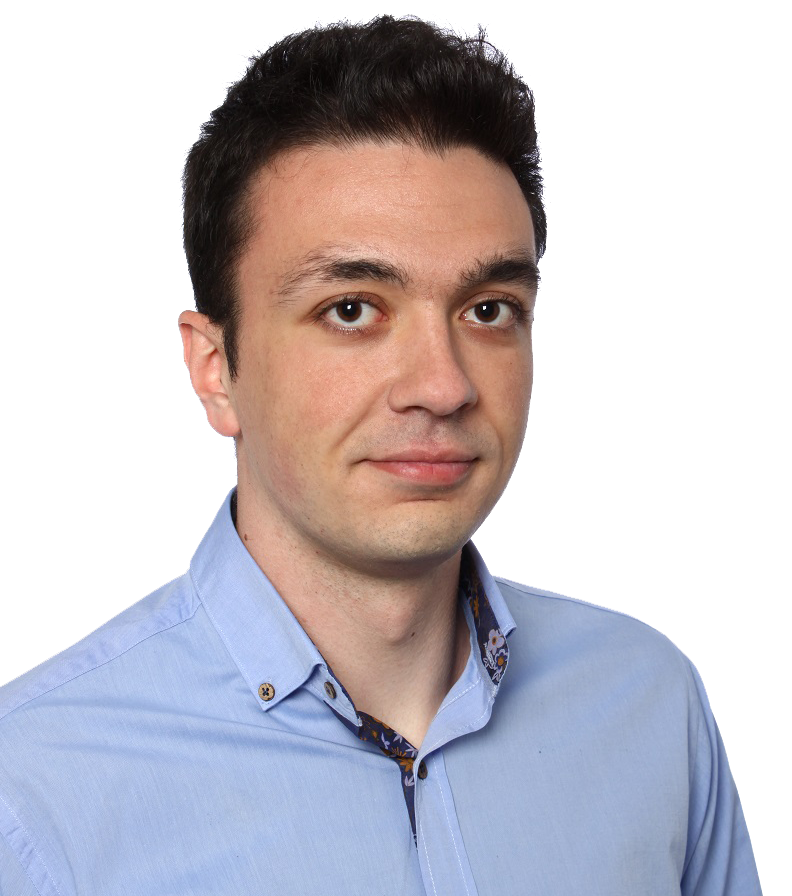
\includegraphics[scale=0.2]{photo.jpg}
		\end{flushright}
	\end{minipage}
	%
	\vspace*{-0.75cm}
	%
	\section{Education}
	
	\begin{EntryDatedLogo}{University of Western Macedonia}{http://icte.uowm.gr}{2012 -- 2017}{Master degree (5 years of study), Dept. of Informatics and Telecomunications Engineering}{-1.25cm}{uowm}{0.6}
		\begin{Itemize}
			%\item Recognized as integrated master degree (level 7 of EFQ) under government gazette 3987/14-9-2018
			%\item Thesis title: "\textit{Design of Market Mechanism for Dynamic Bandwidth Allocation on XG-PON}".
			\item Game theory on XG-PON networks: \url{https://christos.pw/thesis}.
			\item Graduation Grade: 8.2/10.
		\end{Itemize}
	\end{EntryDatedLogo}
	
	\section{Experience}
		\begin{EntryDatedLogo}{Public Power Corporation}{https://www.dei.gr/en}{May 2018 - Now}{Research assistant}{-1.25cm}{dei}{0.6}
		\begin{Itemize}
			\item Researcher on Horizon 2020 programmes (SPEAR, SDN-microSENSE).
			\item Smart grids, industrial networking and cybersecurity.
		\end{Itemize}
	\end{EntryDatedLogo}
	
	\vspace*{0.5cm}
	
	\begin{EntryDatedLogo}{IEK ALFA (Vocational school)}{https://iekalfa.gr}{Oct. 2018 - Jun. 2019}{Teacher}{-1cm}{alfa}{0.6}
		\begin{Itemize}
			\item Computer networks and telecommunications oriented lessons.
			\item Operating Systems and Object-oriented programming (C++).
		\end{Itemize}
	\end{EntryDatedLogo}

	\vspace*{0.5cm}
		
	\begin{EntryDatedLogo}{University of Brighton}{https://www.brighton.ac.uk}{Jul. - Sept. 2017}{Research assistant}{-0.45cm}{brighton}{0.6}
	%	\begin{Itemize}
	%		\item Research on XG-PON and NG-PON2 networks.
	%		\item Development of NG-PON2 simulator in MATLAB.
	%		\item Worked on a novel MAC algorithm for NG-PON2.	
%	\end{Itemize}
	\end{EntryDatedLogo}

	\vspace*{0.5cm}	

	\begin{EntryDatedLogo}{University of Western Macedonia}{http://icte.uowm.gr}{Mar. 2017 - Nov. 2019}{Teaching Assistant}{-1cm}{uowm}{0.6}
	\begin{Itemize}
		\item Computer Networks II, Computer and Network Security.
		\item Event-driven simulation.
	\end{Itemize}
	\end{EntryDatedLogo}

	\vspace*{0.75cm}	

	\begin{EntryDatedLogo}{IntelliSolutions S.A}{http://intelli-corp.com}{Jul. - Aug. 2016}{Systems and Network Engineer (Intern)}{-0.4cm}{intelli}{0.75}
	%\begin{Itemize}
	%	\item Design and implementation of new enterprise network.
	%	\item Network security planning and implementation (pfSense, OpenVPN, firewall, squid).
	%	\item Windows Server, Active Directory and SQL failover cluster setup, type 2 virtualization (VMware).
	%\end{Itemize}
	\end{EntryDatedLogo}
	\newpage
	\section{Skills}
	\begin{tabular}{m{4.5cm} m{13cm}}\renewcommand{\arraystretch}{2}
		\textbf{Telecommunications}   	& ITU-T PONs, Traffic Engineering, Simulation (OmNET++). \\
		\textbf{Networking}   			& CCNA Curriculum, Open vSwitch, RouterOS, ArubaOS, OpenFlow, Ryu SDN controller.\\
		\textbf{Security}				& TLS, PKI, OpenVPN, pfSense, ACLs. \\
		\textbf{System Administration}	& Unix, LEMP stack, Windows Server, Active Directory. \\
		\textbf{Virtualization}			& Xen (XCP-ng), ESXi, Proxmox, VMware/Virtualbox, Docker.\\ 
		\textbf{Programming} 	    	& Java, MATLAB, Python, C/C++, Basics of web development. \\
		\textbf{Miscellaneous}			& Troubleshooting, Project Management, Office Suite, MS Visio, \LaTeX. \\
		\textbf{Languages} 				& Greek (native), English (C2), German (C1). 
	\end{tabular}
	
	\section{Publications}
	\pubentry{1}{C. Dalamagkas, P. Sarigiannidis, S. Kapetanakis and I. Moscholios, "Dynamic scheduling in {TWDM}-{PONs} using game theory", \textit{Optical Switching and Networking}, Dec. 2017, DOI: \href{https://doi.org/10.1016/j.osn.2017.12.004}{\texttt{10.1016/j.osn.2017.12.004}}.}{2018}
	
	\pubentry{2}{C. Dalamagkas, P. Sarigiannidis, I. Moscholios, T. Lagkas and M.S. Obaidat, "PAS: A Fair Game-Driven DBA Scheme for XG-PON Systems", \textit{11th International Symposium on Communication Systems, Networks, and Digital Signal Processing}, Jul. 2018. DOI: 
	\href{https://doi.org/10.1109/CSNDSP.2018.8471787}{\texttt{10.1109/CSNDSP.2018.8471787}}}{2018}
	
	\pubentry{3}{C. Dalamagkas et al., “A Survey On Honeypots, Honeynets And Their Applications On Smart Grid,” in 2019 IEEE Conference on Network Softwarization (NetSoft), 2019. DOI: 
	\href{http://dx.doi.org/10.1109/NETSOFT.2019.8806693}{\texttt{10.1109/NETSOFT.2019.8806693}}}{2019}
	
	\vspace{-0.25cm}
	\section{Professional Certifications}
	\begin{EntryDatedLogo}{Cisco Certified Network Associate (CCNA)}{https://www.cisco.com/}{\scshape{Jul. 2019}}{}{-0.75cm}{cisco}{0.6}
	\end{EntryDatedLogo}
	\vspace{0.25cm}
	
	\section{Voluntary Activities and Memberships}
	\vspace*{0.125cm}	
	\begin{EntryDatedLogo}{University of Western Macedonia}{https://uowm.gr}{Mar. 2016 - Now}{Editor of educational material}{-1.1cm}{uowm}{0.6}
	\begin{Itemize}
		\item Author of original education material for the course "Network Design".
		\item Curriculum includes Cisco and Mikrotik routing and switching.
	\end{Itemize}
	\end{EntryDatedLogo}

	\vspace*{0.5cm}
	
	\begin{EntryDatedLogo}{Institute of Electrical and Electronics Engineers}{https://www.ieee.org/}{Sep. 2013 -- Now}{IEEE Communications Society member}{-0.5cm}{ieee}{0.6}
	\end{EntryDatedLogo}

\end{document}
